\documentclass[
11pt, % The default document font size, options: 10pt, 11pt, 12pt
%codirector, % Uncomment to add a codirector to the title page
]{charter} 




% El títulos de la memoria, se usa en la carátula y se puede usar el cualquier lugar del documento con el comando \ttitle
\titulo{Desarrollo de un dispositivo embebido localizador y botón antipánico} 

% Nombre del posgrado, se usa en la carátula y se puede usar el cualquier lugar del documento con el comando \degreename
% \posgrado{Carrera de Especialización en Sistemas Embebidos} 
\posgrado{Carrera de Especialización en Internet de las Cosas} 
%\posgrado{Carrera de Especialización en Intelegencia Artificial}
%\posgrado{Maestría en Sistemas Embebidos} 
%\posgrado{Maestría en Internet de las cosas}

% Tu nombre, se puede usar el cualquier lugar del documento con el comando \authorname
\autor{Ing. Erik Hromek} 

% El nombre del director y co-director, se puede usar el cualquier lugar del documento con el comando \supname y \cosupname y \pertesupname y \pertecosupname
\director{Mg. Ing. Lucas Dórdolo}
\pertenenciaDirector{FIUBA} 
% FIXME:NO IMPLEMENTADO EL CODIRECTOR ni su pertenencia
%\codirector{Por definir} % para que aparezca en la portada se debe descomentar la opción codirector en el documentclass
%\pertenenciaCoDirector{Por definir}

% Nombre del cliente, quien va a aprobar los resultados del proyecto, se puede usar con el comando \clientename y \empclientename
\cliente{???}
\empresaCliente{???}

% Nombre y pertenencia de los jurados, se pueden usar el cualquier lugar del documento con el comando \jurunoname, \jurdosname y \jurtresname y \perteunoname, \pertedosname y \pertetresname.
%\juradoUno{Nombre y Apellido (1)}
%\pertenenciaJurUno{pertenencia (1)} 
%\juradoDos{Nombre y Apellido (2)}
%\pertenenciaJurDos{pertenencia (2)}
%\juradoTres{Nombre y Apellido (3)}
%\pertenenciaJurTres{pertenencia (3)}
 
\fechaINICIO{20 de junio de 2023}		%Fecha de inicio de la cursada de GdP \fechaInicioName
\fechaFINALPlan{08 de agosto de 2023} 	%Fecha de final de cursada de GdP
\fechaFINALTrabajo{???}	%Fecha de defensa pública del trabajo final


\begin{document}

\maketitle
\thispagestyle{empty}
\pagebreak


\thispagestyle{empty}
{\setlength{\parskip}{0pt}
\tableofcontents{}
}
\pagebreak


\section*{Registros de cambios}
\label{sec:registro}


\begin{table}[ht]
\label{tab:registro}
\centering
\begin{tabularx}{\linewidth}{@{}|c|X|c|@{}}
\hline
\rowcolor[HTML]{C0C0C0} 
Revisión & \multicolumn{1}{c|}{\cellcolor[HTML]{C0C0C0}Detalles de los cambios realizados} & Fecha      \\ \hline
0      & Creación del documento                                 & 20/06/2023 \\ \hline
1      & Se completa hasta el punto 5 inclusive                 & 04/07/2023 \\ \hline
2          & Se aplican correcciones hasta el punto 5 inclusive                  & 09/07/2023 \\ \hline
3          & Se completa hasta el punto 9 inclusive                 & 11/07/2023 \\ \hline
4          & Se aplican correcciones hasta el punto 9 inclusive                & 13/07/2023 \\ \hline
5          & Se completa hasta el punto 12 inclusive y se corrige fecha de finalización & 22/07/2023 \\ \hline
6          & Se aplican correcciones hasta el punto 12 inclusive & 29/07/2023 \\ \hline
7          & Se completa hasta el punto 15 inclusive & 01/08/2023 \\ \hline

%2      & Se completa hasta el punto 7 inclusive
%		  Se puede agregar algo más \newline
%		  En distintas líneas \newline
%		  Así                                                    & dd/mm/aaaa \\ \hline
%3      & Se completa hasta el punto 11 inclusive                & dd/mm/aaaa \\ \hline
%4      & Se completa el plan	                                 & dd/mm/aaaa \\ \hline
\end{tabularx}
\end{table}

\pagebreak



\section*{Acta de constitución del proyecto}
\label{sec:acta}

\begin{flushright}
Buenos Aires, \fechaInicioName
\end{flushright}

\vspace{2cm}

Por medio de la presente se acuerda con el \authorname\hspace{1px} que su Trabajo Final de la \degreename\hspace{1px} se titulará ``\ttitle'', consistirá esencialmente en la implementación de un prototipo de un botón antipánico y localizador, y tendrá un presupuesto preliminar estimado de \textcolor{red}{600} h de trabajo y \textcolor{red}{\$XXX}, con fecha de inicio el \fechaInicioName\hspace{1px} y fecha de presentación pública \fechaFinalName.

Se adjunta a esta acta la planificación inicial.

\vfill

% Esta parte se construye sola con la información que hayan cargado en el preámbulo del documento y no debe modificarla
\begin{table}[ht]
\centering
\begin{tabular}{ccc}
\begin{tabular}[c]{@{}c@{}}Dr. Ing. Ariel Lutenberg \\ Director posgrado FIUBA\end{tabular} & \hspace{2cm} & \begin{tabular}[c]{@{}c@{}}\clientename \\ \empclientename \end{tabular} \vspace{2.5cm} \\ 
\multicolumn{3}{c}{\begin{tabular}[c]{@{}c@{}} \supname \\ Director del Trabajo Final\end{tabular}} \vspace{2.5cm} \\
%\begin{tabular}[c]{@{}c@{}}\jurunoname \\ Jurado del Trabajo Final\end{tabular}     &  & \begin{tabular}[c]{@{}c@{}}\jurdosname\\ Jurado del Trabajo Final\end{tabular}  \vspace{2.5cm}  \\
%\multicolumn{3}{c}{\begin{tabular}[c]{@{}c@{}} \jurtresname\\ Jurado del Trabajo Final\end{tabular}} \vspace{.5cm}                                                                     
\end{tabular}
\end{table}




\section{1. Descripción técnica-conceptual del proyecto a realizar}
\label{sec:descripcion}


El proyecto consiste, en primer lugar, en la investigación y el desarrollo de un prototipo de un dispositivo localizador que funcione como botón antipánico. En segundo lugar, incluye la implementación de una prueba de concepto de una aplicación web que permita recibir y registrar las activaciones del botón antipánico.

Resulta importante realizar una introducción al contexto en el cual se desarrolla este proyecto. Esto permitirá entender los motivos originales del autor, desafíos técnicos del proyecto y las consideraciones/restricciones de este.
El autor tiene experiencia en la adquisición, configuración, implementación y soporte de botones antipánico disponibles en el mercado. Se observa que varios de estos presentan los siguientes inconvenientes:
\begin{itemize}
	\item Especificaciones de hardware obsoletas.
	\item Documentación escasa, desactualizada o incluso incorrecta en algunos casos.
	\item Poca fiabilidad de dispositivo (dificultad para configurarlos, mala señal, desconfianza al momento de utilizarlo).
	\item Inconsistencias entre dispositivos idénticos.
	\item Poca duración de batería (desde aproximadamente 24 horas hasta 3 o 4 días como máximo, cuando lo deseable para el beneficiario final del botón es de al menos 5 o 6 días).
	\item Precio exageradamente elevado y muchas dificultades para adquirirlos mediante proveedores.
	\item Nulas características de seguridad.
\end{itemize}

Se ha investigado y revisado diferentes alternativas en el mercado, así como también se ha trabajado con dispositivos utilizados por sistemas de la competencia llegando a conclusiones similares: no se encuentran dispositivos aceptables cuyo costo sea accesible. 
Por ello, uno de los principales motivos del proyecto es lograr construir un dispositivo que permita validar las elecciones tecnológicas y tener una fiabilidad superior, en comparación con los dispositivos disponibles en el mercado.

Descrito el contexto en el cual se encuentra el proyecto a desarrollar, es de interés realizar una breve introducción de los componentes involucrados. En la figura 1 se observan los componentes con los que contará, como mínimo, el prototipo a construir:
\begin{itemize}
	\item Microcontrolador: permitirá el desarrollo del sistema embebido.
	\item Módulo de telefonía móvil: permitirá conectividad y comunicación mediante SMS y redes IP.
	\item Batería: servirá para el uso del dispositivo de forma autónoma.
	\item Módulo GNSS (\textit{Global Navigation Satellite System}): obtendrá la ubicación geográfica del usuario del botón.
	\item Almacenamiento: permitirá el guardado de la configuración y parámetros del dispositivo.
	\item Activador: actuador físico que disparará una alerta y notificar al sistema web.
\end{itemize}

Adicionalmente, se encuentran algunos componentes web a incorporar en el marco del proyecto:

\begin{itemize}
	\item API receptora de SMS: permitirá la recepción de mensajes del texto del dispositivo y enviarlos a otro sistema.
	\item Aplicación web de seguimiento: aplicación compuesta por un \textit{backend} y un \textit{frontend} que posibilitará registrar y almacenar las alertas.
	\item Base de datos: funcionará como almacenamiento persistente de la aplicación web anterior.
\end{itemize}

Estos componentes se utilizarán a modo de prueba de concepto para probar el correcto funcionamiento del prototipo del botón. También funcionarán como caso de uso para integrar este dispositivo a cualquier plataforma web de similares características.

\begin{figure}[htpb]
\centering 
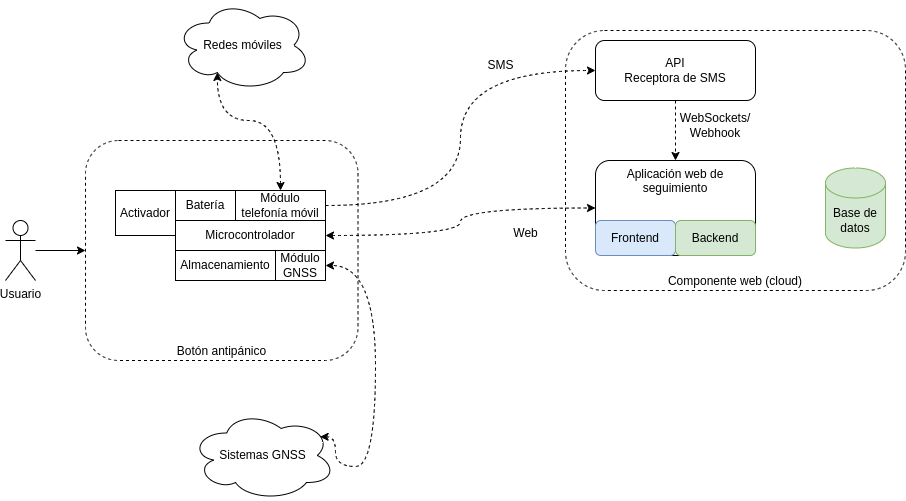
\includegraphics[width=1\textwidth]{./Figuras/diagBloques.png}
\caption{Diagrama en bloques del dispositivo y los componentes web a desarrollar.}
\label{fig:diagBloques}
\end{figure}

\section{2. Identificación y análisis de los interesados}
\label{sec:interesados}

\begin{table}[ht]
%\caption{Identificación de los interesados}
%\label{tab:interesados}
\begin{tabularx}{\linewidth}{@{}|l|X|X|l|@{}}
\hline
\rowcolor[HTML]{C0C0C0} 
Rol           & Nombre y Apellido & Organización 	& Puesto 	\\ \hline
Responsable   & \authorname       & FIUBA        	& Alumno 	\\ \hline
Orientador    & \supname	      & \pertesupname 	& Director Trabajo final \\ \hline
Usuario Final    & Ciudadano & - 	& - \\ \hline
\end{tabularx}
\end{table}


\begin{itemize}
	\item Responsable: principal interesado en la implementación exitosa del dispositivo, posee interés en continuar con el trabajo en futuras etapas.
	\item Orientador: el director posee experiencia dirigiendo aplicaciones con características similares, pero no posee una gran disponibilidad para colaborar; debe acudirse a él solamente con cuestiones muy focalizadas
\end{itemize}


\section{3. Propósito del proyecto}
\label{sec:proposito}

El propósito de este proyecto es validar la idea de que es posible implementar, al menos de forma inicial, un dispositivo que funcione como botón antipánico y localizador. Se busca lograr que este dispositivo permita notificar la ubicación del usuario final al momento de ser activado vía SMS o web y que además trabaje de forma autónoma con una batería.

\section{4. Alcance del proyecto}
\label{sec:alcance}

Para la realización de este proyecto se llevará a cabo:
\begin{itemize}
	\item Una investigación preliminar con relación a los componentes a utilizar.
	\item La implementación del hardware del botón antipánico.
	\item El desarrollo del firmware o software para controlar el dispositivo.
	\item El desarrollo de una plataforma web para recibir las activaciones del botón antipánico.
\end{itemize}

La implementación del dispositivo incluirá:
\begin{itemize}
	\item Conectividad mediante redes móviles.
	\item El uso de un módulo de posicionamiento satelital para tomar la ubicación actual de la persona.
	\item Un mecanismo de configuración/parametrización del dispositivo que sea persistente.
\end{itemize}
Además, contará con alimentación mediante una batería de prestaciones acordes al tamaño del dispositivo y se realizará una investigación acerca del consumo energético de este.

El desarrollo de la plataforma web incluirá la implementación de un servicio online que permita recepcionar mensajes de texto desde teléfonos de Argentina, el registro y visualización de las alertas, a modo de prueba de concepto.

Este proyecto no incluirá:
\begin{itemize}
	\item Aplicación web productiva para gestionar las activaciones del botón antipánico. Por productiva se refiere a que pueda ser ofrecida al mercado o utilizable por usuarios encargados del monitoreo.
	\item Desarrollo de un dispositivo listo para ser lanzado al mercado, es decir que no sea un prototipo.
	\item Desarrollo de un contenedor para el dispositivo.
\end{itemize}

\section{5. Supuestos del proyecto}
\label{sec:supuestos}

\begin{itemize}
	\item Todos los componentes de hardware a utilizar serán definidos luego de una investigación preliminar.
	\item Se intentará utilizar parte del material aprendido durante el curso de especialización relacionado a la programación de sistemas embebidos (bibliotecas, firmware, etc.).
	\item Se utilizará un microcontrolador que pueda ser adquirido a un costo relativamente bajo.
	\item Se contará con un chip de telefonía móvil para utilizar en el proyecto.
	\item Se adquirirán: un módulo de localización satelital, una batería compatible, un módulo de telefonía móvil y un pulsador que estén disponibles en el mercado local.
	\item Para recibir los SMS, se contratará un servicio web que permita recibir los mensajes y redireccionarlos a la aplicación web.

\end{itemize}

\section{6. Requerimientos}
\label{sec:requerimientos}

Los requerimientos se listan agrupados por afinidad:

\begin{enumerate}
\item Grupo de requerimientos del dispositivo geolocalizador:
	\begin{enumerate}
	\item Contar una batería recargable que dure al menos 120 horas (5 días) y sea cargable mediante un cable \textit{Micro USB}.
	\item Contar con botones para encendido/apagado y activación de una alerta.
	\item Tener un indicador del estado del dispositivo: encendido/apagado, señal de telefonía móvil, señal de GPS y nivel de batería.
	\item Contar con conectividad a la red de telefonía móvil.
	\item Obtener periódicamente la ubicación actual del dispositivo y guardarla internamente.
	\item Permitir configurar un número de teléfono para enviar una alerta por mensaje de texto.
	\item Tener un mecanismo de notificación cuando se dispare una alerta, mediante vibración o sonido.
	\item Incluir la ubicación del dispositivo en el mensaje de alerta.
	\item Poder configurar un número de teléfono como administrador del dispositivo.
	\item Permitir configurar parámetros necesarios para el funcionamiento del dispositivo, por ejemplo, datos de la red de telefonía móvil.
	\item Contar con almacenamiento persistente para la configuración.
	\end{enumerate}
\item Grupo de requerimientos asociados al sistema web de gestión de dispositivos y alertas:
	\begin{enumerate}
	\item Recibir y almacenar las alertas enviadas a un número de teléfono designado.
	\item Permitir crear usuarios administradores.
	\item Contar con un acceso web para poder cargar nuevos dispositivos y visualizar alertas.
	\item Contar con una sección para visualizar y exportar el historial de alertas de un dispositivo.
	\item Impedir que un dispositivo no habilitado envíe alertas al sistema.
	\item Debe poder ser desplegable en un entorno \textit{cloud} u \textit{on-premise}.
	\end{enumerate}
\item Grupo de requerimientos de documentación:
	\begin{enumerate}
	\item Incluir un \textit{datasheet} del dispositivo que permita la integración del dispositivo a otros sistemas web.
	\item Incorporar un manual de configuración del dispositivo.
	\item Contar con una licencia de código abierto para el dispositivo.
	\end{enumerate}
\end{enumerate}

\section{7. Historias de usuarios (\textit{Product backlog})}
\label{sec:backlog}

Respecto al peso, se asignarán los valores de acuerdo con una escala basada en la sucesión de Fibonacci, siendo 1 el valor más bajo y 21 el valor más alto, representando este número una tarea extremadamente compleja.

\begin{itemize}
	\item Como usuario del dispositivo deseo poder visualizar el estado de: el dispositivo, la batería, la señal de telefonía móvil y la señal de GPS. Valor: 13.
	\item Como usuario del dispositivo quiero que este tenga un botón físico para encender y apagar el dispositivo. Valor: 5.
	\item Como usuario del dispositivo deseo poder disparar una alerta mediante un botón y recibir una notificación del dispositivo indicando que se disparó la alerta: Valor: 5.
	\item Como usuario del dispositivo deseo poder cargar el dispositivo con un cargador similar al de los teléfonos móviles para poder utilizarlo en cualquier lugar. Valor: 5.
	\item Como usuario administrador quiero poder configurar un teléfono asociado a un dispositivo para que reporte alertas hacia el número designado. Valor: 3.
	\item Como usuario administrador quiero poder recuperar la configuración actual del dispositivo para saber cómo está configurado actualmente. Valor: 3.
	\item Como usuario administrador quiero poder limitar quién puede configurar el dispositivo para que solamente yo pueda modificar su funcionamiento. Valor: 5.
	\item Como usuario administrador quiero poder ingresar a la plataforma web mediante un \textit{login} para hacer uso de esta. Valor: 5.
	\item Como usuario administrador quiero poder crear nuevos usuarios para que tengan acceso a la plataforma web. Valor: 3.
	\item Como usuario administrador quiero poder dar de alta dispositivos para utilizar como botones antipánico. Valor: 5.
	\item Como usuario administrador quiero poder recibir, visualizar y almacenar en tiempo real las alertas recibidas en el sistema web para gestionarlas. Valor: 13.
	\item Como usuario administrador quiero poder visualizar y exportar un reporte de alertas de un dispositivo para tener la información por fuera del sistema web. Valor: 8.
	\item Como usuario administrador quiero contar con un manual de los dispositivos para poder configurarlos. Valor: 3.

\end{itemize}


\section{8. Entregables principales del proyecto}
\label{sec:entregables}


Los entregables del proyecto son:

\begin{itemize}
	\item Prototipo de dispositivo geolocalizador.
	\item Aplicación web desplegada en un entorno \textit{cloud}.
	\item Código fuente del firmware del dispositivo.
	\item Código fuente de la aplicación web.
	\item Documentación asociada a la aplicación web.
	\item Manual del dispositivo.
	\item Informe final.
\end{itemize}

\section{9. Desglose del trabajo en tareas}
\label{sec:wbs}


\begin{enumerate}
\item Planificación del proyecto (46 h)
	\begin{enumerate}
	\item Definición de requerimientos (10 h)
	\item Armado de la planificación (32 h)
	\item Revisión de la planificación (2 h)
	\item Revisión de requerimientos con el director (2 h)
	\end{enumerate}
\item Investigación previa (60 h)
	\begin{enumerate}
	\item Investigación de microcontrolador y plataforma a usar (8 h)
	\item Investigación de módulos y sensores a adquirir (12 h)
	\item Análisis del consumo de energía del dispositivo y los módulos (8 h)
	\item Investigación y comparación de proveedores \textit{cloud} (8 h)
	\item Análisis de tecnologías web (8 h)
	\item Investigación de servicios para interfaz web receptora de SMS (12 h)
	\item Definición de entornos de desarrollo para la programación embebida y web (4 h)
	\end{enumerate}
\item Desarrollo e implementación de dispositivo embebido (134 h)
	\begin{enumerate}
	\item \textit{Setup} inicial del firmware (6 h)
	\item Realizar diagrama esquemático del dispositivo y sus módulos (8 h)
	\item Realizar pruebas iniciales de conexión del dispositivo y sus módulos (8 h)
	\item Desarrollo del sistema asociado al módulo de telefonía móvil (16 h)
	\item Desarrollo del sistema asociado al módulo de localización satelital (12 h)
	\item Desarrollo del sistema asociado al módulo de configuración y almacenamiento de parámetros (16 h)
	\item Desarrollo del sistema asociado a la gestión del estado del dispositivo (20 h)
	\item Desarrollo del sistema asociado al módulo de alertas (12 h)
	\item Desarrollo del sistema asociado al manejo de batería y energía del dispositivo (16 h)
	\item Integración entre todos los módulos al sistema operativo de tiempo real (20 h)
	\end{enumerate}
\item Desarrollo y despliegue de sistema web (209 h)
	\begin{enumerate}
	\item Armado de modelo de datos (12 h)
	\item Armado de maquetas funcionales para interfaz de usuario (8 h)
	\item \textit{Setup} inicial del \textit{backend} (4 h)
	\item Desarrollo de módulo de gestión de usuarios (16 h)
	\item Desarrollo de módulo de gestión de dispositivos (16 h)
	\item Implementación de módulo de recepción de alertas (20 h)
	\item Desarrollo de módulo de gestión de alertas (20 h)
	\item Implementación de pruebas unitarias generales del \textit{backend} (20 h)
	\item \textit{Setup} inicial del \textit{frontend} (2 h)
	\item Desarrollo de interfaces de usuario de administración (25 h)
	\item Desarrollo de interfaz de usuario para gestión de alertas (40 h)
	\item Integración al \textit{backend} y pruebas de interfaces de usuario (20 h)
	\item Despliegue de sistema web (6 h)
	\end{enumerate}
\item Pruebas de funcionamiento del sistema (58 h)
	\begin{enumerate}
	\item Pruebas del dispositivo (30 h)
	    \begin{enumerate}
	    \item Pruebas de funcionamiento de la conexión del dispositivo a la red de telefonía móvil (4 h)
	    \item Pruebas de funcionamiento de la localización satelital del dispositivo (4 h)
	    \item Pruebas de funcionamiento del dispositivo con los indicadores de estado (4 h)
	    \item Pruebas de funcionamiento de las alertas del dispositivo (4 h)
	    \item Pruebas de funcionamiento de la configuración persistente del dispositivo (4 h)	
	    \item Pruebas de funcionamiento de la duración de la batería (8 h)
	    \item Pruebas de funcionamiento del dispositivo con el actuador de encedido (2 h)
	    \end{enumerate}
	\item Pruebas del sistema web (28 h)
	    \begin{enumerate}
	    \item Pruebas de funcionamiento de creación y edición de usuarios (6 h)
	    \item Pruebas de funcionamiento de creación y edición de dispositivos (6 h)
	    \item Pruebas de funcionamiento de módulo de gestión de alertas (8 h)
	    \item Pruebas de circuito completo del dispositivo y la plataforma (8 h)
	    \end{enumerate}
	\end{enumerate}
\item Elaboración de documentación y manuales (36 h)
	\begin{enumerate}
	\item Elaboración del manual del dispositivo (20 h)
	\item Elaboración de documentación del sistema web (16 h)
	\end{enumerate}
\item Elaboración de documentación del proyecto (60 h)
	\begin{enumerate}
	\item Elaboración de la memoria técnica del proyecto (40 h)
	\item Elaboración de la presentación del proyecto (20 h)
	\end{enumerate}
\end{enumerate}

Cantidad total de horas estimadas: 603 h

\section{10. Diagrama de Activity On Node}
\label{sec:AoN}

El camino crítico, como se observa en la figura 2, es de 433 horas.

\begin{figure}[htpb]
\centering 
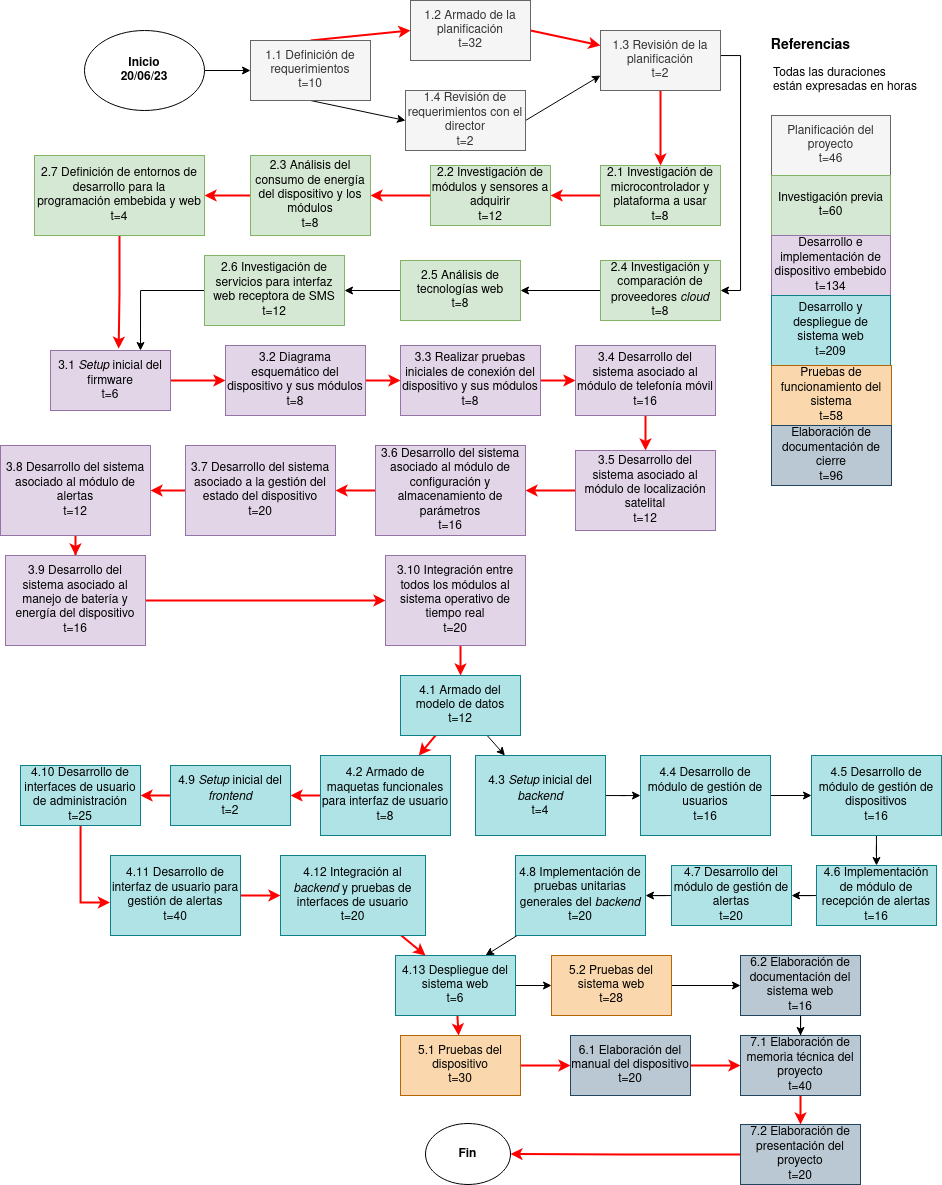
\includegraphics[width=.9\textwidth]{./Figuras/AoN.png}
\caption{Diagrama de \textit{Activity on Node}.}
\label{fig:AoN}
\end{figure}

Nota: no se desglosaron las actividades correspondientes a las pruebas del dispositivo (5.1) y pruebas del sistema web (5.2) para no ocupar complejizar el gráfico de \textit{Activity On Node} pero estas están todas relacionadas entre sí.

\section{11. Diagrama de Gantt}
\label{sec:gantt}

En la figura 3, se muestra el desglose de actividades del proyecto y en las figuras 4, 5 y 6 se presenta todo el plan de actividades ordenado en el tiempo.

El cronograma de las actividades está planificado a razón de 25 horas de dedicación semanal, posterior a la finalización de la planificación.
 
\begin{figure}[htpb]
\centering 
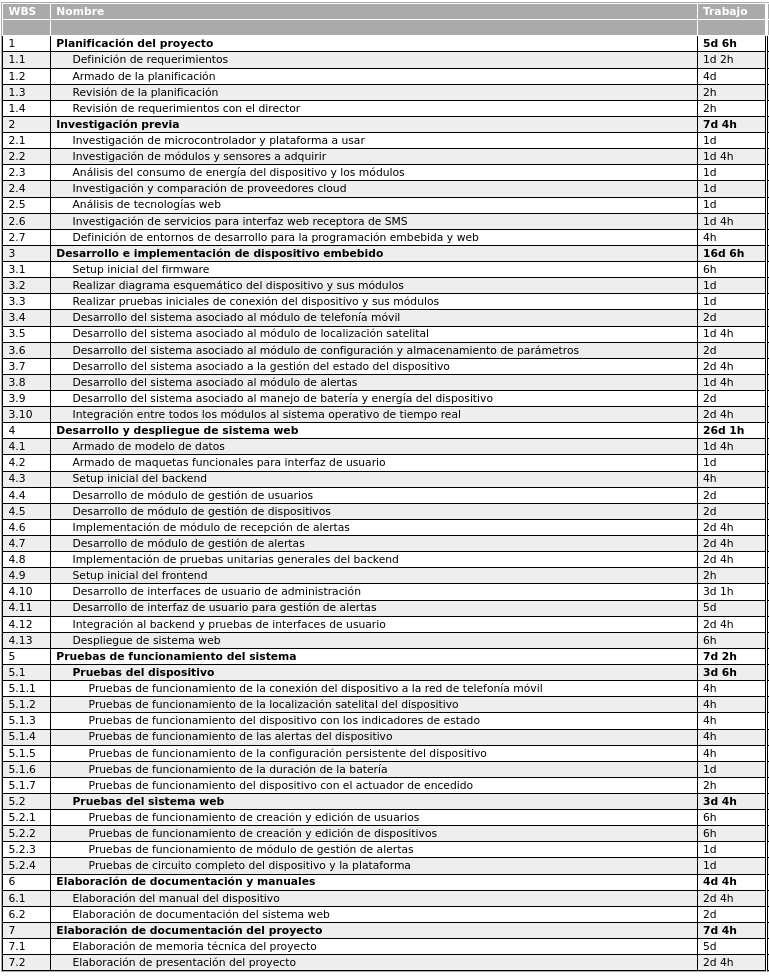
\includegraphics[width=.9\textwidth]{./Figuras/WBS.png}
\caption{Desglose de actividades del proyecto.}
\label{fig:diagGanttWBS}
\end{figure}

\begin{landscape}
\begin{figure}[htpb]
\centering 
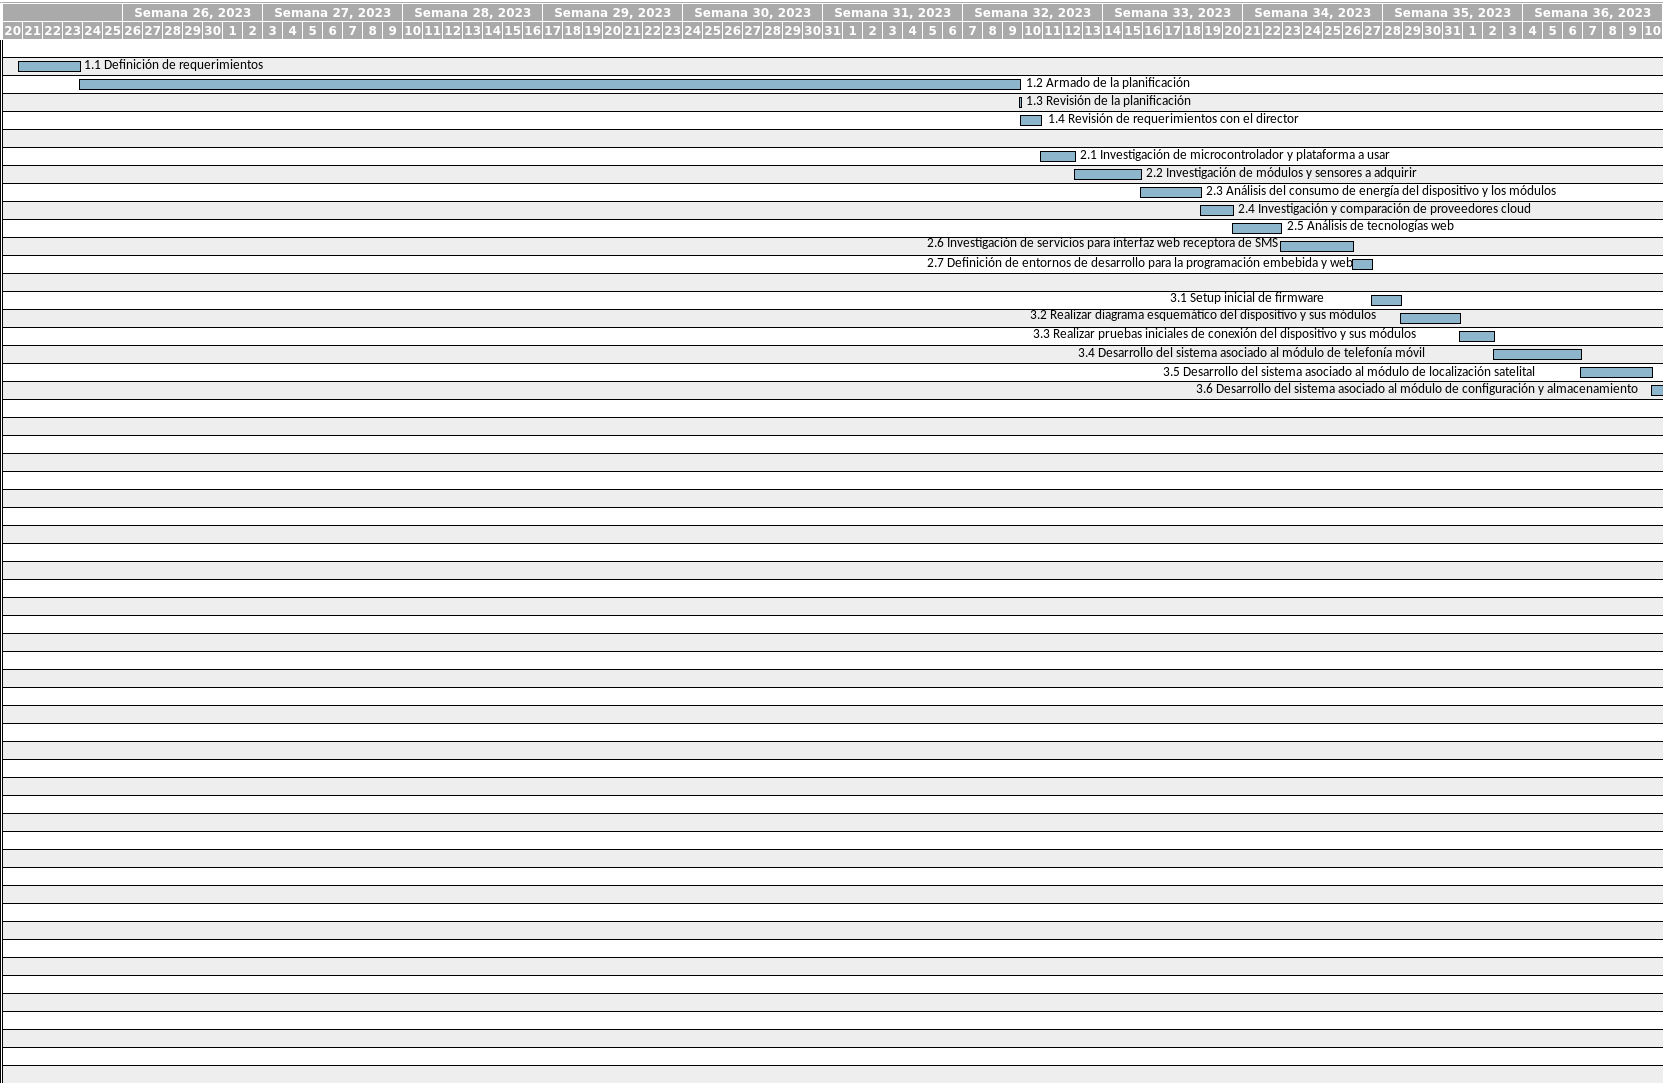
\includegraphics[width=\paperwidth]{./Figuras/Gantt1.png}
\caption{Diagrama de Gantt del proyecto (primera parte).}
\label{fig:diagGantt1}
\end{figure}
\end{landscape}

\begin{landscape}
\begin{figure}[htpb]
\centering 
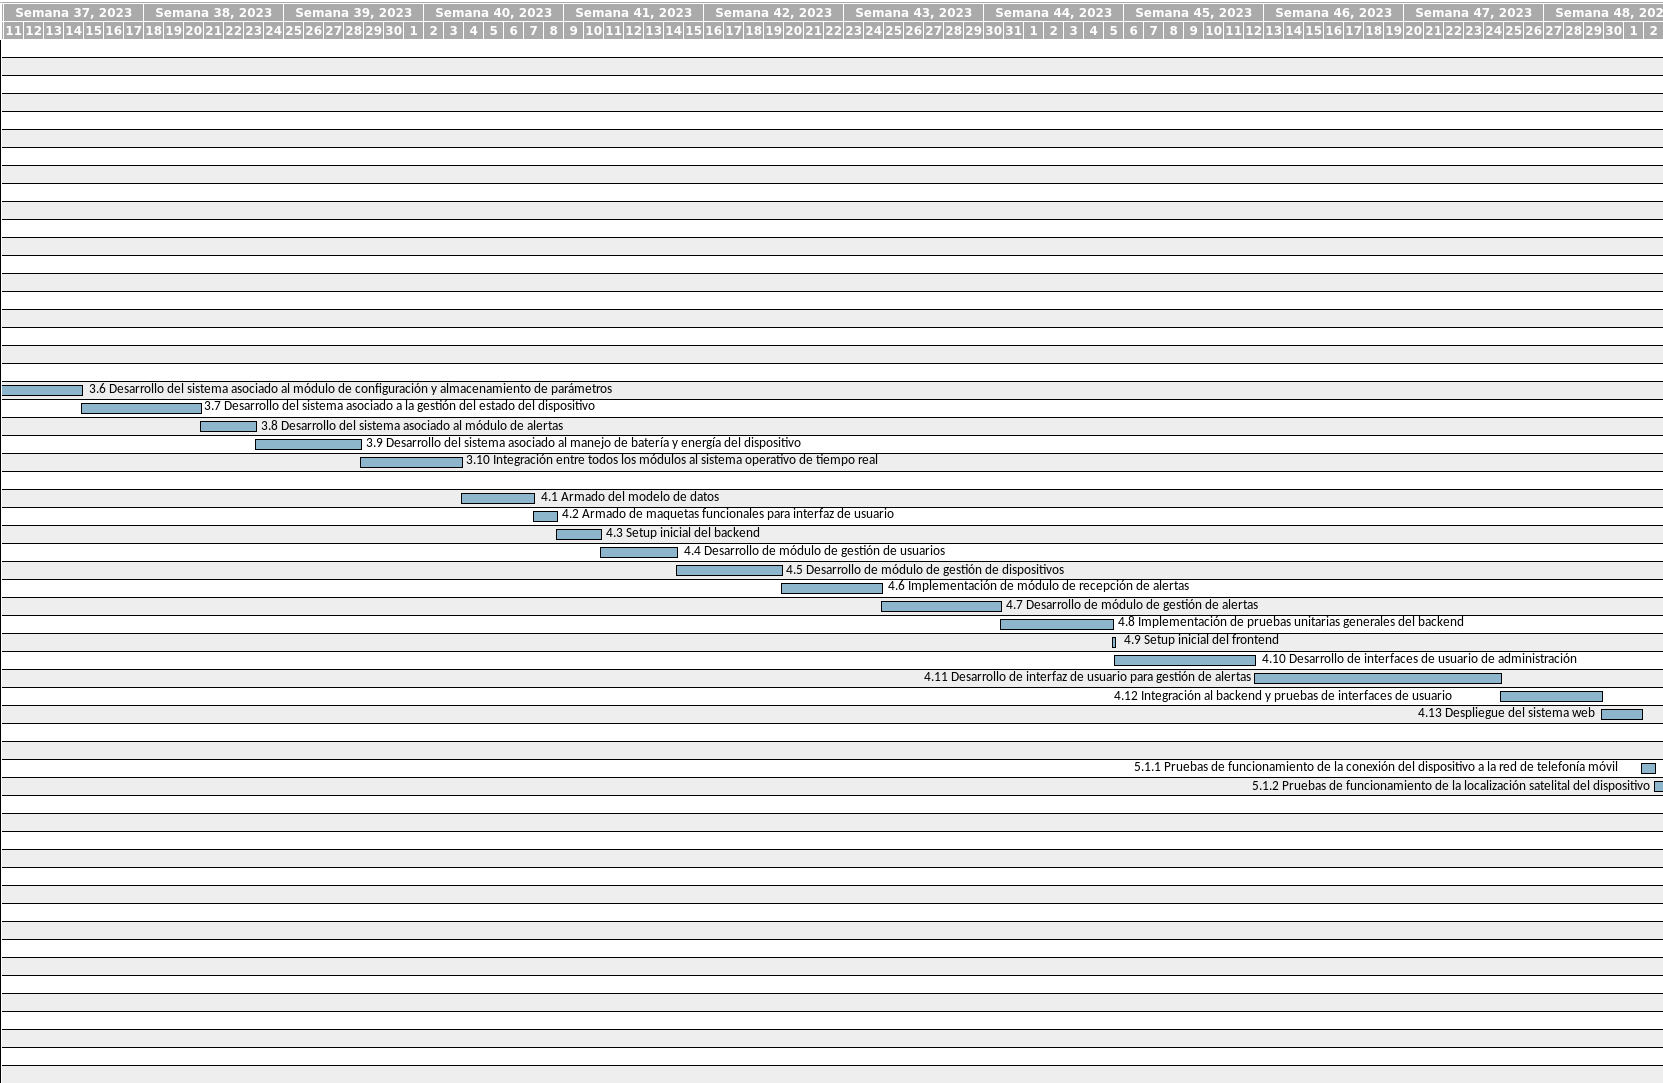
\includegraphics[width=\paperwidth]{./Figuras/Gantt2.png}
\caption{Diagrama de Gantt del proyecto (segunda parte).}
\label{fig:diagGantt2}
\end{figure}
\end{landscape}

\begin{landscape}
\begin{figure}[htpb]
\centering 
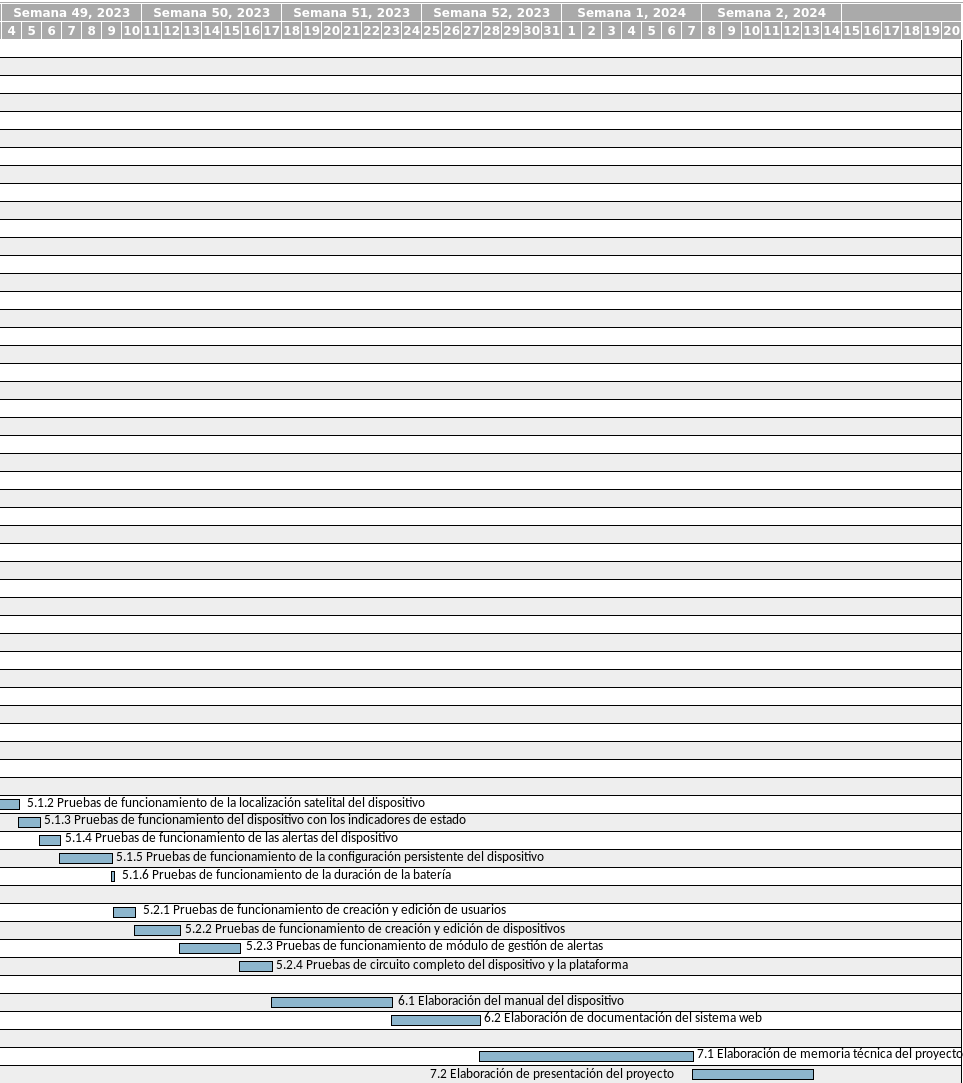
\includegraphics[height=.9\textheight]{./Figuras/Gantt3.png}
\caption{Diagrama de Gantt del proyecto (tercera parte).}
\label{fig:diagGantt3}
\end{figure}
\end{landscape}


\section{12. Presupuesto detallado del proyecto}
\label{sec:presupuesto}

Los costos se encuentran expresados en pesos argentinos (ARS).

\begin{table}[htpb]
\centering
\begin{tabularx}{\linewidth}{@{}|X|c|r|r|@{}}
\hline
\rowcolor[HTML]{C0C0C0} 
\multicolumn{4}{|c|}{\cellcolor[HTML]{C0C0C0}COSTOS DIRECTOS} \\ \hline
\rowcolor[HTML]{C0C0C0} 
Descripción &
  \multicolumn{1}{c|}{\cellcolor[HTML]{C0C0C0}Cantidad} &
  \multicolumn{1}{c|}{\cellcolor[HTML]{C0C0C0}Valor unitario} &
  \multicolumn{1}{c|}{\cellcolor[HTML]{C0C0C0}Valor total} \\ \hline
 Horas ingeniero Jr. &
  \multicolumn{1}{c|}{603} &
  \multicolumn{1}{c|}{1500} &
  \multicolumn{1}{c|}{904500} \\ \hline
 Microcontrolador &
  \multicolumn{1}{c|}{1} &
  \multicolumn{1}{c|}{6000} &
  \multicolumn{1}{c|}{6000} \\ \hline
 Batería &
  \multicolumn{1}{c|}{1} &
  \multicolumn{1}{c|}{4000} &
  \multicolumn{1}{c|}{4000} \\ \hline
  Módulo telefonía móvil &
  \multicolumn{1}{c|}{1} &
  \multicolumn{1}{c|}{6000} &
  \multicolumn{1}{c|}{6000} \\ \hline
  
  Módulo GPS &
  \multicolumn{1}{c|}{1} &
  \multicolumn{1}{c|}{6000} &
  \multicolumn{1}{c|}{6000} \\ \hline
  
  Chip telefonía móvil &
  \multicolumn{1}{c|}{1} &
  \multicolumn{1}{c|}{1000} &
  \multicolumn{1}{c|}{1000} \\ \hline
  
  Accesorios varios &
  \multicolumn{1}{c|}{1} &
  \multicolumn{1}{c|}{20000} &
  \multicolumn{1}{c|}{20000} \\ \hline
  
  Alojamiento \textit{cloud} &
  \multicolumn{1}{c|}{1} &
  \multicolumn{1}{c|}{15000} &
  \multicolumn{1}{c|}{15000} \\ \hline
  
  API \textit{cloud} para telefonía &
  \multicolumn{1}{c|}{1} &
  \multicolumn{1}{c|}{10000} &
  \multicolumn{1}{c|}{10000} \\ \hline
  
\multicolumn{3}{|c|}{SUBTOTAL} &
  \multicolumn{1}{c|}{972500} \\ \hline
\rowcolor[HTML]{C0C0C0} 
\multicolumn{4}{|c|}{\cellcolor[HTML]{C0C0C0}COSTOS INDIRECTOS} \\ \hline
\rowcolor[HTML]{C0C0C0} 
Descripción &
  \multicolumn{1}{c|}{\cellcolor[HTML]{C0C0C0}Cantidad} &
  \multicolumn{1}{c|}{\cellcolor[HTML]{C0C0C0}Valor unitario} &
  \multicolumn{1}{c|}{\cellcolor[HTML]{C0C0C0}Valor total} \\ \hline
\multicolumn{1}{|l|}{10\% de los costos directos} &
   \multicolumn{1}{|c|}{1} &
   \multicolumn{1}{|c|}{97250} & 
   \multicolumn{1}{|c|}{97250} \\ \hline
\multicolumn{3}{|c|}{SUBTOTAL} &
  \multicolumn{1}{c|}{97250} \\ \hline
\rowcolor[HTML]{C0C0C0}
\multicolumn{3}{|c|}{TOTAL} &
   1069750\\ \hline
\end{tabularx}%
\end{table}

Nota: los costos de los componentes de hardware y los servicios \textit{cloud} son aproximados; se tomó un valor aproximado en base a una revisión de posibles módulos y servicios candidatos al momento de la elaboración de la planificación. Respeto al ítem de accesorios, se refiere a cables, conectores, y otros elementos que se deban adquirir para la implementación del prototipo de hardware.

\section{13. Gestión de riesgos}
\label{sec:riesgos}

a) Identificación de los riesgos más importantes analizados y la estimación de sus consecuencias:

Riesgo 1: no cumplir con el plan de trabajo dentro de los tiempos estipulados por demoras en las actividades o poca dedicación horaria.
\begin{itemize}
	\item Severidad (8): la severidad es muy alta porque incide en la fecha de finalización del proyecto y el tiempo disponible para presentar todo el trabajo final.
	\item Probabilidad de ocurrencia (5): es posible que ocurra por otros compromisos laborales que puedan surgir o por inconvenientes encontrados durante el desarrollo del proyecto.
\end{itemize}   

Riesgo 2: no contar con documentación suficiente y bibliotecas de desarrollo adecuadas de los módulos de hardware.
\begin{itemize}
	\item Severidad (7):  la severidad es alta porque obliga a dedicar más tiempo a analizar y entender el funcionamiento de los módulos o incluso tener que desarrollar más funcionalidades, generando demoras.
	\item Ocurrencia (6): la probabilidad de ocurrencia es considerable ya que es algo común con este tipo de componentes y los fabricantes, ya que pueden o no haber disponibilizado bibliotecas actualizadas para las plataformas de desarrollo.
\end{itemize}

Riesgo 3: tener dificultad para interactuar y configurar correctamente el módulo de telefonía móvil.
\begin{itemize}
	\item Severidad (5): la severidad es moderada ya que si bien puede implicar mayor dedicación de tiempo a este módulo, es solamente uno de tantos del proyecto.
	\item Ocurrencia (6): la probabilidad de ocurrencia es cuantiosa ya que no resulta trivial la interacción y correcto uso de estos módulos, puesto que tienen muchos cambios de estados.
\end{itemize}

Riesgo 4: encontrarse con dificultad para interactuar y configurar correctamente el módulo de localización satelital.
\begin{itemize}
	\item Severidad (5): la severidad es moderada ya que si bien puede implicar mayor dedicación de tiempo a este módulo, es solamente uno de tantos del proyecto.
	\item Ocurrencia (6): la probabilidad de ocurrencia es cuantiosa ya que no resulta trivial la interacción y correcto uso de estos módulos, puesto que tienen muchos cambios de estados.
\end{itemize}

Riesgo 5: tener demoras en la obtención/entrega de módulos de hardware.
\begin{itemize}
	\item Severidad (5): la severidad es moderada ya que implicaría una posible demora en las pruebas iniciales de interacción con los módulos de hardware, pero el tiempo podría ocuparse adelantando otras actividades del desarrollo web.
	\item Ocurrencia (3): la probabilidad es baja ya que existen varias alternativas de módulos en el mercado local.
\end{itemize}

Riesgo 6: presentar dificultades en el desarrollo del \textit{frontend} de la aplicación web.
\begin{itemize}
	\item Severidad (5): la severidad es moderada puesto que podría implicar asignar más horas al desarrollo de \textit{frontend} y sus posteriores pruebas y validaciones.
	\item Ocurrencia (7): la probabilidad de ocurrencia es alta ya que actualmente no se cuenta con tanta experiencia y habilidades en el uso de \textit{frameworks} web modernos.
\end{itemize}

Riesgo 7: inconvenientes para contar con un servicio de recepción de mensajes de texto.
\begin{itemize}
	\item Severidad (8): la importancia de este riesgo es muy alta ya que impediría recibir los mensajes de texto de alerta, y obligaría a buscar un método alternativo de comunicación con el botón antipánico.
	\item Ocurrencia (5): la probabilidad de ocurrencia no es alta ya que existen varios servicios de este estilo, pero podrían tener inconvenientes para operar en el país.
\end{itemize}

Riesgo 8: no lograr tener una duración de batería aceptable para el prototipo.
\begin{itemize}
	\item Severidad (6): la severidad es considerable ya que impacta con uno de los principales objetivos del proyecto, que es contar con una duración de batería superior a varios días.
	\item Ocurrencia (6): es probable que ocurra, dependiendo del tamaño de la batería adquirida y de las medidas que se puedan aplicar dentro del desarrollo.
\end{itemize}

Riesgo 9: superar el costo esperado de los componentes en comparación de soluciones del mercado.
\begin{itemize}
	\item Severidad (5): el peso de este riesgo no es tan alto, porque si bien es muy deseable poder disminuir al máximo los costos de los componentes, también debe tenerse en cuenta que en esta etapa es preferible adquirir componentes que simplifiquen y agilicen el trabajo, aunque tengan un mayor costo.
	\item Ocurrencia (6): existen probabilidades de que ocurra debido a varios factores, entre los que se encuentran los costos de importación en aumento y el hecho de querer preferir módulos más adecuados para el armado del prototipo.
\end{itemize}

b) Tabla de gestión de riesgos:

\begin{table}[htpb]
\centering
\begin{tabularx}{\linewidth}{@{}|X|c|c|c|c|c|c|@{}}
\hline
\rowcolor[HTML]{C0C0C0} 
Riesgo & S & O & RPN & S* & O* & RPN* \\ \hline
1. No cumplir con el plan de trabajo dentro de los tiempos estipulados por demoras en las actividades o poca dedicación horaria.       & 8  & 5  &  40   & 8  & 3  & 24   \\ \hline
2. No contar con documentación suficiente y bibliotecas de desarrollo adecuadas de los módulos de hardware.      & 7  & 6  &  42   & 5  & 4  & 20   \\ \hline
3. Tener dificultad para interactuar y configurar correctamente el módulo de telefonía móvil.       & 5  & 6  &  30   & 5  & 3  & 15   \\ \hline
4. Encontrarse con dificultad para interactuar y configurar correctamente el módulo de localización satelital.      & 5  & 6  &  30   & 5  & 3  & 15   \\ \hline
5. Tener demoras en la obtención/entrega de módulos de hardware.       & 5  & 3  &  15   &    &    &      \\ \hline
6. Presentar dificultades en el desarrollo del \textit{frontend} de la aplicación web.      & 5  & 7  &  35   & 4  & 5  & 20   \\ \hline
7. Inconvenientes para contar con un servicio de recepción de mensajes de texto.       & 8  & 5  &  40   & 8  & 3  & 24   \\ \hline
8. No lograr tener una duración de batería aceptable para el prototipo.       & 6  & 6  &  36   & 4  & 4  & 16   \\ \hline
9. Superar el costo esperado de los componentes en comparación de soluciones del mercado.     & 5  & 6  &  30   & 3  & 6  & 18   \\ \hline
\end{tabularx}%
\end{table}

Criterio adoptado: 
Se tomarán medidas de mitigación en los riesgos cuyos números de RPN sean mayores a 25.

Nota: los valores marcados con (*) en la tabla corresponden luego de haber aplicado la mitigación.

c) Plan de mitigación de los riesgos que originalmente excedían el RPN máximo establecido:
 
Riesgo 1: No cumplir con el plan de trabajo dentro de los tiempos estipulados por demoras en las actividades o poca dedicación horaria.
\begin{itemize}
	\item Plan de mitigación: dedicar como mínimo las horas planteadas en el plan de trabajo, asignar mayor horas de trabajo en el quinto bimestre del año actual ya que no se cursarán materias y no aceptar otros compromisos laborales.
	\item Severidad (8): la severidad se mantiene igual.
	\item Probabilidad de ocurrencia (3): la probabilidad de tener atrasos significativos por falta de dedicación horaria se achica bastante, además de que se pretende poder asignar más horas mientras no se cursen materias adicionales.
\end{itemize}

Riesgo 2: no contar con documentación suficiente y bibliotecas de desarrollo adecuadas de los módulos de hardware.
\begin{itemize}
	\item Plan de mitigación: hacer foco durante la etapa de investigación en la disponibilidad de documentación y compatibilidad; validar con el director del trabajo por recomendación de componentes.
	\item Severidad (5): la severidad se reduce ya que se se contará indefectiblemente con bibliotecas actualizadas y documentación disponibles para todos los componentes de hardware que se pueda.
	\item Probabilidad de ocurrencia (4): la probabilidad de tener atrasos significativos por falta de dedicación horaria se achica bastante, además de que se pretende poder asignar más horas mientras no se cursen materias adicionales.
\end{itemize}
 
Riesgo 3: tener dificultad para interactuar y configurar correctamente el módulo de telefonía móvil.
\begin{itemize}
	\item Plan de mitigación: se validarán los módulos de telefonía móvil con el director y se tendrá en cuenta la gestión de estados posibles del módulo.
	\item Severidad (5):  la severidad se mantiene igual debido a la importancia de este módulo.
	\item Probabilidad de ocurrencia (3): la probabilidad de que ocurra y genere demoras se reduce ya que se tendrán en cuenta de entrada consideraciones sobre el uso de los módulos de telefonía móvil.
\end{itemize}

Riesgo 4: encontrarse con dificultad para interactuar y configurar correctamente el módulo de localización satelital.
\begin{itemize}
	\item Plan de mitigación: se validarán los módulos de localización satelital con el director y se tendrá en cuenta la gestión de estados posibles del módulo.
	\item Severidad (5):  la severidad se mantiene igual debido a la importancia del módulo.
	\item Probabilidad de ocurrencia (3): la probabilidad de que ocurra y genere demoras se reduce ya que se tendrán en cuenta de entrada consideraciones sobre el uso de los módulos de localización satelital y su interacción con el microcontrolador.
\end{itemize}

Riesgo 6: presentar dificultades en el desarrollo del \textit{frontend} de la aplicación web.
\begin{itemize}
	\item Plan de mitigación: se buscará en la investigación inicial tecnologías que simplifiquen el desarrollo de \textit{frontend} y la visualización de datos en tiempo real y se intentara contar con apoyo/asistencia externa a modo de soporte por trabas en el desarrollo.
	\item Severidad (4): se reduce el peso de la severidad ya que se intentará utilizar técnologías que puedan brindar de antemano ciertas facilidades para el desarrollo de \textit{frontend}.
	\item Probabilidad de ocurrencia (5): al preseleccionar un \textit{framework} o tecnología que ya haya sido estudiado se espera disminuir la posibilidad de tener demoras/retrasos en el desarrollo de \textit{frontend}.
\end{itemize}

Riesgo 7: inconvenientes para contar con un servicio de recepción de mensajes de texto.
\begin{itemize}
	\item Plan de mitigación: se buscarán servicios nacionales e internacionales que puedan proveer esta funcionalidad durante la etapa de investigación inicial, en el caso de que un proveedor no este disponible o sus características no sean acordes para este proyecto. 
	\item Severidad (8): la severidad se mantiene igual.
	\item Probabilidad de ocurrencia (3): la probabilidad de no poder contar con ninguna alternativa para poder recibir y leer mensajes de texto desde el sistema web se reduce considerablemente ya que existen muchas aplicaciones que hacen uso de este tipo de servicios.
\end{itemize}

Riesgo 8: no lograr tener una duración de batería aceptable para el prototipo.
\begin{itemize}
	\item Plan de mitigación: se analizará de que forma de puede reducir el consumo de batería de los módulos mediante técnicas de ahorro de batería y reposo del microcontrolador y los módulos. Además, se tendrán en cuenta baterías de mayor capacidad, y por lo tanto mayor costo, que sean compatibles para que más adelante se sepa que es posible contar con una mayor autonomía.
	\item Severidad (4): se disminuye la severidad ya que se tendrá la posibilidad de adquirir baterías de similar funcionamiento, es decir que sea compatibles, pero de mayor capacidad. A fines de lograr tener el prototipo es aceptable saber que se podrá extender el tamaño de la batería.
	\item Probabilidad de ocurrencia (4): se disminuye la probabilidad de impacto porque se aprovechará de forma más eficiente el consumo de energía de los dispositivos.
\end{itemize}

Riesgo 9: superar el costo esperado de los componentes en comparación de soluciones del mercado.
\begin{itemize}
	\item Plan de mitigación: se tendrán en cuenta durante la investigación componentes que sean compatibles con los elegidos, pero tengan un menor costo debido a que no vengan con facilidades para el desarrollo, como por ejemplo pines de conectividad.
	\item Severidad (3): se disminuye la severidad ya que se tendrá en cuenta un listado de componentes que tengan compatibilidad o igual funcionamiento, pero que puedan ser más complejos de incorporar al prototipo o conectar con los demás módulos.
	\item Probabilidad de ocurrencia (6): la probabilidad de ocurrencia se mantiene igual, ya que es preferible pagar un mayor costo por componentes que ya vengan conectados o tengan facilidades para el desarrollo.
\end{itemize}

\section{14. Gestión de la calidad}
\label{sec:calidad}

Se listarán a continuación los requerimientos que, desde el punto de vista del responsable del proyecto, su relevancia es mayor para el desarrollo del prototipo:

\begin{itemize} 
\item Req \#1.1: contar una batería recargable que dure al menos 120 horas (5 días) y sea cargable mediante un cable Micro USB.

\begin{itemize}
	\item Verificación: se calculará el consumo energético aproximado del prototipo para saber cuanto debe ser el tamaño de la batería y se implementarán formas de optimizar el consumo energético dentro del desarrollo.
	\item Validación: se dejará funcionando el prototipo durante el mayor tiempo posible y se verificará la carga de batería.
\end{itemize}

\item Req \#1.2: contar con botones para encendido/apagado y activación de una alerta.

\begin{itemize}
	\item Verificación: se incorporarán actuadores físicos para el dispositivo y se verificará que sea correcta la lógica para que cada uno tenga su correspondiente acción.
	\item Validación: se probará cada uno reiteradas veces para validar su función.
\end{itemize}

\item Req \#1.4: contar con conectividad a la red de telefonía móvil.

\begin{itemize}
	\item Verificación: se analizará el desarrollo y revisará el funcionamiento del módulo de gestión de conectividad a la red de telefonía móvil mediante una máquina de estados.
	\item Validación: se verificará que el dispositivo reciba y envíe mensajes y que detecte correctamente el número de teléfono del chip usado.
\end{itemize}

\item Req \#1.6: permitir configurar un número de teléfono para enviar una alerta por mensaje de texto.

\begin{itemize}
	\item Verificación: se chequeará que el \textit{firmware} del dispositivo guarde el teléfono configurado mediante revisión de código.
	\item Validación: se chequeará que el mensaje de alerta llegue al teléfono indicado y que su información sea correcta posterior a una prueba de alerta..
\end{itemize}

\item Req \#1.8: incluir la ubicación del dispositivo en el mensaje de alerta.

\begin{itemize}
	\item Verificación: se comprobará que el \textit{firmware} del prototipo envíe siempre la última ubicación registrada en el mensaje de alerta mediante análisis de código.
	\item Validación: se chequeará que el mensaje de alerta contenga exactamente la información esperada luego de una prueba.
\end{itemize}

\item Req \#1.9: poder configurar un número de teléfono como administrador del dispositivo.

\begin{itemize}
	\item Verificación: se comprobará en el código que el dispositivo solamente acepte los comandos del teléfono configurado previamente.
	\item Validación: se validará enviando mensajes desde diferentes números de teléfono.
\end{itemize}

\item Req \#1.11: contar con almacenamiento persistente para la configuración.

\begin{itemize}
	\item Verificación: se comprobará que los parámetros de configuración se almacenen en el microcontrolador.
	\item Validación: se probará reiniciando el dispositivo varias veces para verificar que la configuración sea persistente.
\end{itemize}

\item Req \#2.1: recibir y almacenar las alertas enviadas a un número de teléfono designado.

\begin{itemize}
	\item Verificación: se comprobará en el código que el módulo de telefonía móvil envíe los mensajes de alerta al número configurado y se revisará que el servicio web para recibir mensajes de texto lea en tiempo real los mensajes recibidos.
	\item Validación: se realizarán pruebas de disparos de alerta y se revisará la plataforma web para validar que se visualicen las alertas en tiempo real.
\end{itemize}

\end{itemize}

\begin{itemize}
\item Req \#2.3: contar con un acceso web para poder cargar nuevos dispositivos y visualizar alertas.

\begin{itemize}
	\item Verificación: se verificará que los usuarios creados puedan acceder al sitio.
	\item Validación: se llevarán a cabo pruebas de circuito completo para verificar que los usuarios puedan cargar nuevos dispositivos y acceder el módulo de visualización de alertas.
\end{itemize}

\item Req \#2.4: contar con una sección para visualizar y exportar el historial de alertas de un dispositivo.

\begin{itemize}
	\item Verificación: se verificará que los usuarios creados puedan acceder a la sección de visualización de alertas.
	\item Validación: se llevarán a cabo pruebas de circuito completo para verificar que los usuarios puedan visualizar las alertas en tiempo real y exportar los resultados de las pruebas.
\end{itemize}

\item Req \#2.5: impedir que un dispositivo no habilitado envíe alertas al sistema.

\begin{itemize}
	\item Verificación: se analizará la plataforma web y el servicio para recibir mensajes de texto para que no se registren en el sistema mensajes que no correspondan a dispositivos cargados en el sistema. 
	\item Validación: se simularán pruebas de alerta desde otros teléfonos, emulando mensajes de texto de alerta.
\end{itemize}

\item Req \#3.2: incorporar un manual de configuración del dispositivo.

\begin{itemize}
	\item Verificación: se destinará tiempo para la elaboración de un manual de configuración del dispositivo. 
	\item Validación: se validará que el manual contenga pasos necesarios para configurar un dispositivo desde cero.
\end{itemize}

\end{itemize}

\section{15. Procesos de cierre}    
\label{sec:cierre}

Al finalizar el proyecto, se contemplarán las siguientes actividades con sus pautas de trabajo:
\begin{itemize}
	\item Análisis de la ejecución y resultados del plan de trabajo:
	\begin{itemize}
		\item Responsable a cargo: Ing. Erik Hromek. 
		\item Procedimiento: 
		\begin{itemize}
		\item Se analizarán todas las actividades del plan de trabajo original y se compararán los tiempos planificados versus ejecutados.
		\item Se revisarán los objetivos iniciales del proyecto y se determinará el grado de cumplimiento de cada uno.	
		\item Se evaluarán los entregables del proyecto para determinar si son acordes a lo planeado inicialmente.
		\item Se revisará la aplicación del plan de mitigación de riesgos y su impacto en el proyecto.
		\end{itemize}
	\end{itemize}
	\item Análisis de riesgos, inconvenientes, problemas presentados, cambios ocurridos y técnicas y procedimientos útiles:
	\begin{itemize}
		\item Responsable a cargo: Ing. Erik Hromek. 
		\item Procedimiento: 
		\begin{itemize}
		\item Se identificarán los riesgos, inconvenientes y demoras encontradas a lo largo de la ejecución y las medidas adoptadas para su superación.
		\item Se analizarán las técnicas y procedimientos que no fueron planteadas originalmente pero que fueron útiles para el desarrollo de las actividades.
		\item Se identificarán y analizarán los cambios surgidos en el proyecto que alteraron el plan original.
		\end{itemize}
	\end{itemize}
	\item Acto de presentación y agradecimiento a todos los participantes e interesados del proyecto:
	\begin{itemize}
		\item Responsable a cargo: Ing. Erik Hromek. 
		\item Procedimiento: 
		\begin{itemize}
		\item Se hará un agradecimiento al director del proyecto, colaboradores externos, jurados, profesores y autoridades de la carrera de especialización e 					interesados en el proyecto. 
		\end{itemize}
	\end{itemize}
\end{itemize}


\end{document}
